% This is samplepaper.tex, a sample chapter demonstrating the
% LLNCS macro package for Springer Computer Science proceedings;
% Version 2.20 of 2017/10/04
% TEMPLATE: https://www.springer.com/de/it-informatik/lncs/conference-proceedings-guidelines
%
\documentclass[runningheads]{llncs}
%
\usepackage{graphicx}
% Used for displaying a sample figure. If possible, figure files should
% be included in EPS format.
\usepackage{comment}
\usepackage{lettrine} % if you want the first letter to be \letterine{b}{igger}
%
% If you use the hyperref package, please uncomment the following line
% to display URLs in blue roman font according to Springer's eBook style:
% \renewcommand\UrlFont{\color{blue}\rmfamily}

\begin{document}
%
\title{Providing Secrecy for Business Processes running on Blockchain\thanks{Supported by organization x.}}
%
%\titlerunning{Abbreviated paper title}
% If the paper title is too long for the running head, you can set
% an abbreviated paper title here
%
\author{Henry Bergstroem\inst{1} \and
Jan Mensch\inst{2}}
%
\authorrunning{F. Author et al.}
% First names are abbreviated in the running head.
% If there are more than two authors, 'et al.' is used.
%
\begin{comment}
\institute{Princeton University, Princeton NJ 08544, USA \and
Springer Heidelberg, Tiergartenstr. 17, 69121 Heidelberg, Germany
\email{lncs@springer.com}\\
\url{http://www.springer.com/gp/computer-science/lncs} \and
ABC Institute, Rupert-Karls-University Heidelberg, Heidelberg, Germany\\
\email{\{abc,lncs\}@uni-heidelberg.de}}
\end{comment}
%
\maketitle              % typeset the header of the contribution
%
\begin{abstract}
\textbf{\uppercase{how to use bib}} The abstract should briefly summarize the contents of the paper in
15--250 words. Also, this is how you cite stuff \cite{texbook}. Citations are kept in the refs.bib file. You can add citations from google scholar, by clicking on the bibtex link. Then just paste it in the refs.bib file and you are done \cite{web:lang:stats} \cite{latex:companion}. If you want to tell the user on which page you found stuff, do it like this \cite[p.~42]{texbook}. If you are trying to cite stuff that is not there, it will show up like this \cite{kndfljdsjksdjf}.

\keywords{First keyword  \and Second keyword \and Another keyword.}
\end{abstract}

\section{Introduction}
Blockchain is a buzzword that is still very popular today. Mostly it is assoicated with cryptocurreny and token based system such as namecoin \cite{}. With the appearance of Ethereum the capabilities of Blockchain technologies increases drascically since it was now possible to upload turing complete programs called smart contract to the blockchain. In turn many of the exsisting trust related problems can be outsourced to this decentralized system. 
In this paper we are exploring a way of conducing consesus in an active choeography while still protecting the privicy of the participants. The advantage of such sulotuion would be that entities can collaborate with each other while no trust is needed and an immutable protected audit trait can easily be provided to ensure accountability.

\subsection{Introduction to Blockchain \& Ethereum}
The blockchain is a distributed ledger running on multiple machines. The protocol is designed in a way to make every new entery of the ledger...

\subsection{Introduction to BPMN}
It is a buisness model charts and schemas.. old people... glasses.

\subsection{Introduction to Active Choegraphy}
it is the same thing.. more glasses. \cite{weber2016untrusted} prepare for a fat copy-pasta bolognease.

\section{General Problem}
here is quick outlier of how the general problem looks like: 
\begin{itemize}
    \item there are several parties who want to collaborate 
    \item parties have no trust in each other 
    \item parties have no trust in a third party
    \item parties want to collaborate with each other
    \item parties have strong interest in keeping things secret
\end{itemize}

\textbf{example:} Here we give an example, including a BPMN model with the restaurant pizza delivery szenario (relatable).

\subsection{Tradition Solution}
parties have to trust each other 

there is a third party involved

there is one party that controlles everything (a very strong party, e.g. Amazon)


\subsection{Alternative solution with Blockchain Technology}
here we explain how active choreographies work and cite from the paper again \cite{weber2016untrusted}. Also now we have to show that if we choose an active choreography as a solution, there are two possible paths to take: 

\begin{enumerate}
    \item make everything public. We don`t want this to happen. This would be the approach described in \cite{weber2016untrusted}.
    \item have a private blockchain. For that we would have to trust the party, which is hosting that private chain. We don`t like this solution, because we are paranoid. 
    \item use chryptography to keep it hidden in plain sight (our approach).
\end{enumerate}

\section{Approach}
\subsection{Assumptions}
The following assumptions are made: 
\begin{itemize}
    \item the blockchain is public
    \item everyone can see what is posted on the blockchain
    \item an adversary does not trac the traffic from individual participants from and to the blockchain. Therefore if the name of sender of a message is not stored in plain text on the chain, nobody knows who send the message.
    \item the participants of a businesss process (bp) do not trust each other, but would like to cooperate with each other
    \item it is possible to express any bp with a program and this program can enforce the coresponding busieness process
    \item it is possible for a program on the chain to notify a party (avoid busy-wait) 
    \item This program can be viewed as a state-machine
\end{itemize}

\subsection{Ideal solution}
The ideal solution would look something like this: 
\begin{itemize}
    \item process uses a public blockchain
    \item A participant can enable a third trusted party to view all communication (audit trail) if (and only if!) one of the participants of that communication grants that third party permission to do so. Example: A is a supplier, B a seller, C the logistics guy, sending stuff from A to B, E the buyer, who buys stuff from B and F the logistics guy sending stuff from B to E. Something went wrong when ordering the supplies. A is unhappy with this and calls a lawyer. A can provide the lawyer with the audit trail of the communication he was involved in (e.g. between A and B, A and C and between A, B and C) but he can not give the lawyer any other communication, since he himself can not see that.
    \item parties agree on a process and that process has to be executed exactly as specified
    \item the parties only have to communicate via the blockchain
    \item execution of a bp is cheap (cost of gas on etherium)
    \item an observer, who read everything on the public blockchain that is used as a mediator between the parties can not know derive any conclusion about how the business logic looks like (logic), who send what messages when (message) and what messages where send (content).
\end{itemize}


\subsection{Where should the logic of the business process be kept?}


As mentioned before we try to enforce a business process (bp) with an active choreography, while still keeping the content, communication and (in part) the model secret. Since we are in favour of using a public blockchain, we can consider all logic (the model) and all communication that is done with a smart contract running on such a blockchain as public. We could encrypt the messages exchanged between smart contact and the participants of the Business Process. This would keep the content and maybe even the communication secret, but if we keep the logic of the bp public that would be of no use. A simple example to illustrate this point:

\begin{figure}
    \centering
    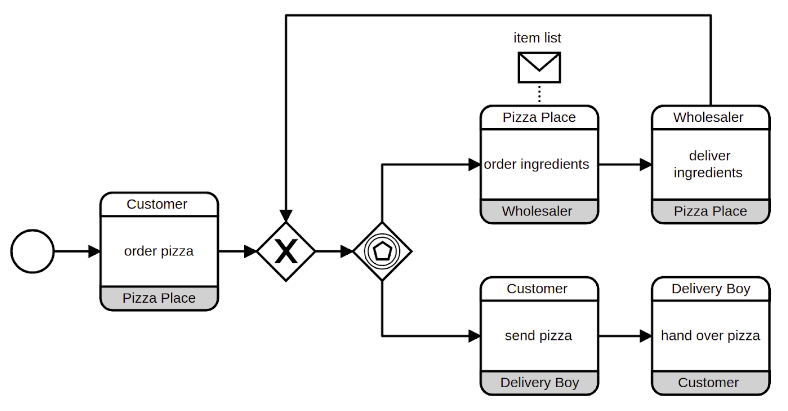
\includegraphics[scale=0.6]{bpmn.png}
    \caption{A simple BPMN}
    \label{fig:bpmn}
\end{figure}

If we implement the bp shown in \ref{fig:bpmn} as an active choreography and put it on a public blockchain there is no point in trying to keep any of the communication secret. What do we mean by that? Let`s assume an observer tracks all communication done with the active choreography, but has no understanding what is being communicated and who is sending which messages. The observer does not need this information to be able to understand all details of the communication. She can just watch the state-changes in the bp. If, for example the state changes to \textit{ordered pizza}, the observer knows that a customer just ordered a pizza. If then changes to \textit{order ingredients}, the observer understands that \textit{Pizza Place} does not have enough ingredients to process that order. Even if we try our best to keep content and communication secret, if we keep the state of the bp public, an outsider might be able to understand who is communicating and what is being communicated. The only thing we might be able to keep secret are mere details about the communication. For this reason we decided to keep the model off-chain. 


\subsection{Implementing an active choreography off-chain}

An active choreography will make sure that a business process is executed as defined. Any attempt by a participant to evoke an illegal state-change will be rejected, since the business process knows what state-changes are legal and under what conditions they are carried out. This approach is no longer possible, if the active choreography is not aware of the business logic. Instead the clients would have to agree on what bp to execute and in which state they are. To keep a record of what business process is executed, the clients could share a hash of that bp (or rather the code representing that process) and store it on the blockchain. 

If a client now wants to execute a state-change in the bp, there should be a consensus among all clients that this state change is legal. If we use a "normal" consensus protocol this would not keep a client from cheating, since the choreography has no knowledge of the consensus. An example: \textit{Customer} wants to order a Margarita pizza. For that he would like to do trigger a state change. For that he drafts the message \textit{Order Margarita for 5 EUR}. If we have a consensus protocol, e.g. based on voting the other clients could now accept or reject that message and with it the state-change. Let`s assume they accept it. \textit{Customer} now sends the message \textit{Order Margarita for 1 EUR} to the active choreography, which, with a client based consensus protocol, has no way of rejecting this message as illegal. 

To prevent this from happening a feasible consensus protocol might like \ref{fig:simple}, with $S_x$ being the secret key of each participant. In our example \textit{customer} drafts the message \textit{Order Margarita for 5 EUR} and encrypts it with his secret key $S_c$. The message is then send of to all other participants. Each of whom encrypt it with their secret key. 


\begin{figure}
    \centering
    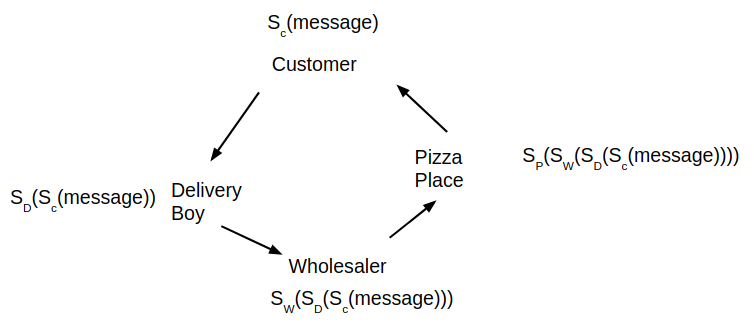
\includegraphics[scale=0.6]{simple_consensus.png}
    \caption{The simple version of the consensus protocol}
    \label{fig:simple}
\end{figure}


At the end the four times encrypted message reaches \textit{customer} again. He than sends it to the active choreography together with the order they were encrypted in and the actual message. The message might look something like this \textit{cipher, message, [C, D, W, P]}. The active choreography is in possession of all public keys. It applies them in order to the received cipher and compares the result with the message it received. If it is the same and all public keys were applied to the message it knows that there was a consensus between all clients. 

What happens in the case of a disagreement? Let`s assume that the actual cost of the Margarita pizza is 6 EUR, not 5 EUR. The \textit{pizza place} on receiving and encrypting  $S_W(S_D(S_C(message)))$ will simply not encrypt it with its own private key. \textit{Customer} has no way to still do a state-change, because the active choreography will reject the message, if it was not encrypted by all participants. 

What happens if \textit{customer} or any other participant tries to cheat? Customer will receive $S_P(S_W(S_D(S_C(message))))$ and can encrypt it. If he replaces \textit{message} with something else, he will fail to encrypt it again, since he is not in possession of the other secret keys. The active choreography will therefore reject the message. The same is true for all other participants. 


\subsection{Advancing the idea of the simple consensus protocol}

There are two obvious drawbacks from the simple consensus protocol displayed in \ref{fig:simple}: 

\begin{enumerate}
    \item In order for the active choreography to be able to reject an invalid message, we have to provide it with the original message, which we would like to agree in order to keep the content of the message secret
    \item Every participant of the bp will know all messages exchanged, even messages which do not affect him. 
    \item An observer will always know who the originator of the message was, since it always is the first client in the provided order. In our example the order was \textit{[C, D, W, P]}, which, in this protocol, makes it obvious that this is a message from the owner of the C key-pair.
\end{enumerate}



\subsection{Circles}



\begin{comment}

\textbf{keep logic secret:} The program $P$, matching the bp should be kept on client side. Since we are just communicating via the Blockchain, the communication of how this process looks like should be done on-chain. For that $P$ should only be stored in encrypted form on the chain. If someone tries to cheat and executes a different program, this will be obvious later, since a record of the actual program (or a hash of it) is kept on-chain. 

\textbf{keep message and content secret:} It should be possible for messages (and logic) to be seen only by parties that are involved in processing those messages. Therefore we need some sort of encrypted "broadcast" of a message within a group. Some of the groups from the example above could be as following (just an example): $G_1 = \{A,B\}$, $G_2 = \{A,C\}$, $G_3 = \{A, B, C\}$, $G_4 = \{E, B, F\}$. So within $G_1$, $G_2$, $G_3$ and $G_4$ we should be able to exchange messages without the other participants (or an outsider) realizing who send a message (secret message) and what was send (secret content). A proposed solution to establish this "encrypted broadcast" for $G_3$ (or any other group): 

\begin{itemize}
    \item A, B, C each generate a key pair. Key pair for A is denoted as public key: $pk_A$, private/secret key $sk_A$. They post it on the chain. The chain now contains $pk_A$, $pk_B$, $pk_C$.
    \item One of the group (lets say A) is chosen as a master. He is kicking off the process
    \item A is now generating a symmetric key $S$
    \item A is posting $pk_B(S)$ (S encrypted by public key of A), $pk_C(S)$  to the chain. B and C now take those values and are thus in position of $S$. Nobody else besides of A, B and C knows $S$
    \item A will post $pk_A(hash(S))$. Everyone can check, if the hash matches up with his/her version of $S$. If it does not, we know that Something went wrong.
    \item If B wants to broadcast in $G_3$ now he is posting $S(sk_B(message), B)$ (his name encrypted with $S$ and the encrypted message encrypted with $S$. This way we know that the message is from B. We do not have to check if the message is from A or C, since it sais that it is from B. Nobody else knows that it is from B, since it is also encoded by $S$. Also nobody knows the content.
\end{itemize}

This process is distributed (no third party needed) and requires no trust. Also the blockchain is only used as storage and there are no cryptographic operations done on-chain, so the operations are (hopefully) affordable.

\textbf{further thoughts:} Since we can view the pb as a state-machine, every state change must be posted to the chain. We can do this with the process described above. State changes have to be reflected on client side. 

\textbf{questions}: Things I am not sure about, that I would like to talk about
\begin{itemize}
    \item Do we need some sort of consensus protocol to make sure that all clients are in the same state?
    \item How do we convert a BPM into code? Are the assumptions correct?
    \item  Is the ideal solution really the ideal solution? 
    \item Does the encryption idea make any sens?
    \item Is there a better way to enforce that the correct program is being executed on client side?
\end{itemize}


\end{comment}


\section{Architecture Alternatives}
We have discussed a range of different alternatives of how the architecture can look like. Each architecture has its advantages and disadvantages.

\textbf{Where to put the code associated with the buissness logic?}
The blockchain acts like the source of truth for the actors. One main question is what is best to keep on the blockchain and what is better off. To maximaze uniforminess between the actors it would make sense to have all logic on the blockchain. The obvious downside with the blockchain is that it is expensive to use and that everything is public. Depending on the buisness cheography and its priorities the better choice might be to leave parts of the buisness logic off-chain. The following table highlight the pros and ons about having the code on or off chain.

\begin{table*}[t]
  \centering
  \begin{tabular}{p{6cm}p{6cm}}
  \hline
    \textbf{On-Chain} & \textbf{off-Chain}\\
    \hline \hline
    
 expensive & cheap \\
     harder to scale & easier to scale \\
     more transparent & more secret \\
     enforcable & not directly enforcable \\

\hline
  \end{tabular}
  \caption{installation options Grafana }
  \label{tab:1}
\end{table*}


\subsubsection{How to make enforce an off-chain choreography}

If we decide to have the code code off-chain, to ensure that the business logic is kept secret, the question is how to ensure that a agreed upon business process will still be executed as specified. Since the smart contract in that case would only save the current state of the business process, it would have no way of knowing which state change would be legal or illegal to execute next. 

An example: 

\textbf{do an example with the food delivery?}

An other example: Alice $A$, Bob $B$ and evil Eve $E$ would like to participate in a business process. $E$ intends to be cheating (meaning not executing the business process in the pre-defined order). All three parties agree on a business process that should be executed. This business process is compiled executable code \textbf{do we even need that?}. To consolidate this, they save a hash of this code on-chain. All parties now start to execute the business process. There are therefore state-changes to the business process. This state changes are reflected on-chain, without or any outsider being aware of the underlying business process. The smart contract thus acts as an interface between the clients and the blockchain, which here plays the role of an audit trail, not an active choreography. If $E$ now sends an illegal state change to be recorded in the audit trail, the smart contract has no way of rejecting that, since it itself does not know if the proposed state change is legal or illegal.

A technique to avoid this is introduced by parity \footnote{https://wiki.parity.io/Private-Transactions}: In their implementation before a client can communicate with the blockchain, it has to validate its communication with a validator. \textit{how does the chain then know that the validator sad that this is ok? Assumption: It will check the signature of the client and the validator and know that this validator is responsible for that client.}. To avoid all this overhead and to make communication more private, we propose to use a ring signature. Ring signatures were first introduced in 2001 by Rivest et al. and make it possible to specify a group of possible signers without giving away who the actual author of a signed message is \ref{rivest2001leak}. Ring signatures are already used in combination with blockchain technology, among others the CrypoNote protocol used in the Monero network \ref{van2013cryptonote}. In the protocol, a participant can not know from whome or to whome he or she is sending money or is receiving money from, only that the sender or receiver is part of a one-time ring signature.



We propose that there exists exactly one ring, which includes all participants (regardless of their circle). If a participant now wants to have a state-change confirmed he/she has it signed by all other participants in the ring. A participant who is in the same circle as the sender can read the message. If he she disagrees with the content of the message (the state-change) he can communicate this back to the sender and prevent the state change. Since the smart contract can check if the message was signed with the ring signature $E$ has no way of submitting an invalid state-change. We now moved from an audit trail to an active choreography. 

There is still an obvious flaw in the proposed implementation: How do we prevent $E$ from halting any state change at any moment? She could just interrupt the continuity of the business process. So far we do not have any good answer to this. We could hope that it is still in the best interest of $E$ that the business process is fully executed and she therefore would not want to interrupt it. A more technical option would be to have the clients generate random messages to confuse $E$, so that it at least would be very hard for her to halt the business process at a certain state. However this is just a suggestion and topic to further research.



How can a client prove to the chain that the propsed state-change is legal?
zero-knowledge?
confirmation of other clients
\bibliographystyle{splncs04} % BibTeX users should specify bibliography style 'splncs04'.
\bibliography{refs} % Entries are in the "refs.bib" file
table

\end{document}
